\subsection{Once-through results}

\begin{frame}
    \frametitle{Reactor numbers scales with the power 
    output of the reactors}
            \begin{itemize}
                \item Scenario 2 (MMR) deploys the most reactors
                \item Scenario 3 (Xe-100) deploys the fewest reactors
                \item Similar number of Xe-100s and VOYGRs are deployed
                \item Scenarios 4 (Xe-100+MMR), 6 (Xe-100+VOYGR), and 7 
                      (Xe-100+VOYGR+MMR) mostly deploy Xe-100s 
                \item Scenario 5 (MMR+VOYGR) mostly deploys VOYGRs
            \end{itemize}
        \vspace{0.2cm}
        \begin{figure}
        \begin{subfigure}{0.48\textwidth}
                \centering
                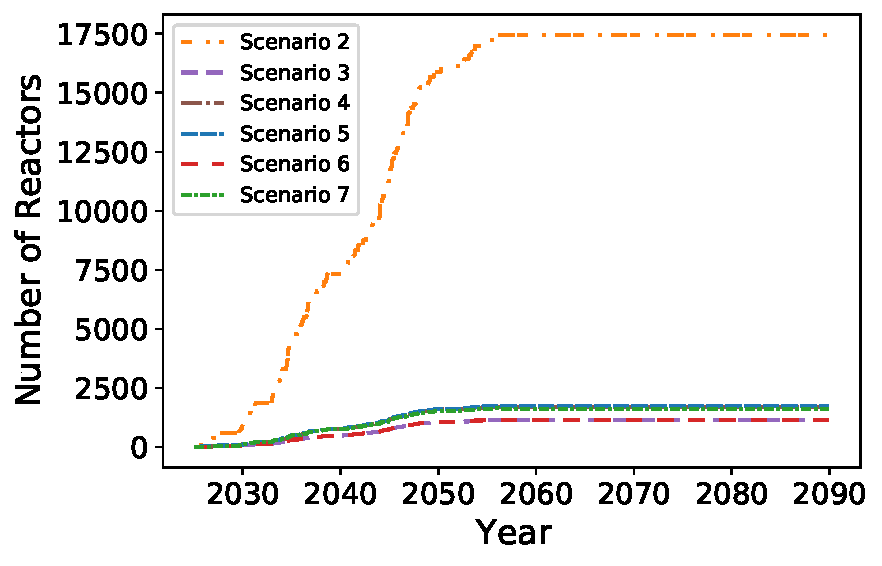
\includegraphics[width=0.88\textwidth]{nogrowth_reactors.pdf}
        \end{subfigure}
        \hfill
        \begin{subfigure}{0.48\textwidth}
            \centering
            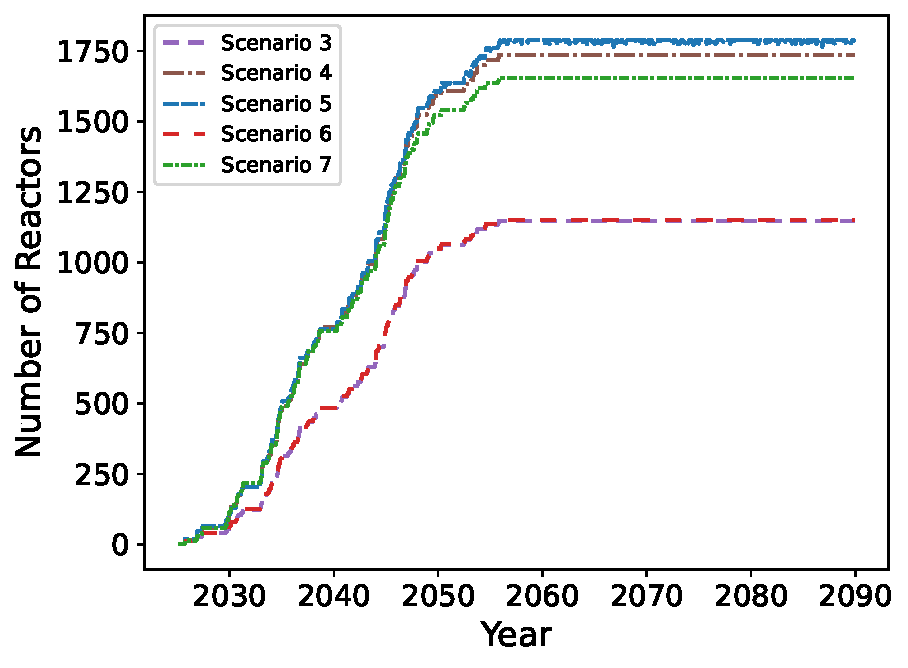
\includegraphics[width=0.88\textwidth]{nogrowth_reactors_3-7.pdf}
        \end{subfigure}
        \vspace{-0.15cm}
        \caption{Number of advanced reactors deployed in Scenarios 2-7 (left)
        and Scenarios 3-7 (right).}
        \end{figure}
\end{frame}

\begin{frame}
    \frametitle{Reactor designs drives the uranium mass required}
    \begin{columns}
        \column[t]{4.5cm}
            \begin{itemize}
                \item Scenario 5 (MMR + VOYGR) requires the largest average mass of 
                      enriched uranium
                \item Scenario 5 (MMR + VOYGR) requires the smallest mass of \gls{HALEU}
                \item Scenario 2 (MMR) requires the largest mass of \gls{HALEU}
                \item Scenario 3 (Xe-100) requires the smallest mass of enriched 
                      uranium
                \end{itemize}
        \column[t]{6.3cm}
        \vspace{-0.8cm}
            \begin{figure}
                \centering
                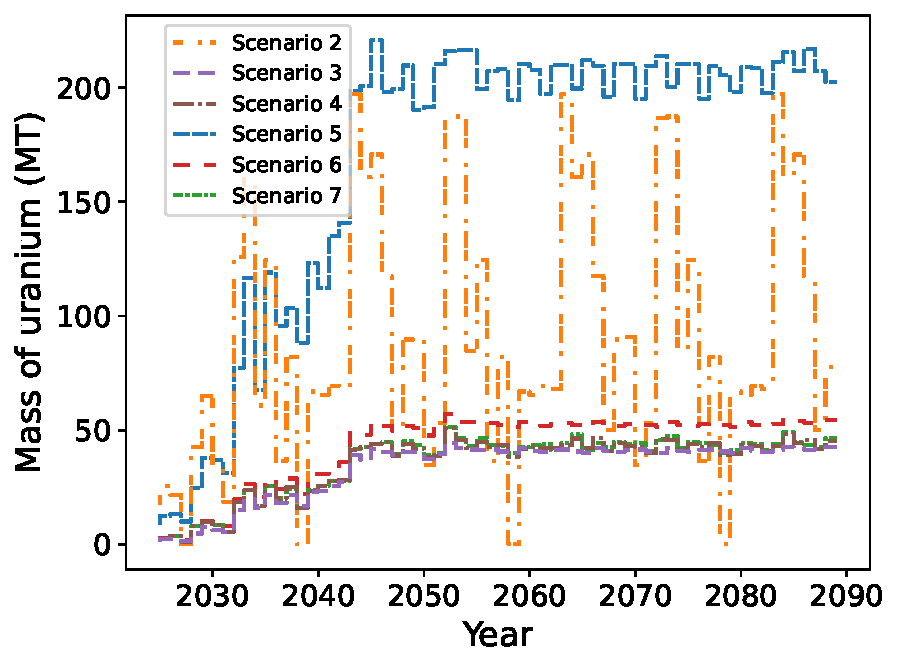
\includegraphics[scale=0.42, trim=5 0 0 0,clip]{nogrowth_AR_uranium.pdf}
                \caption{Annual average mass of enriched uranium required to fuel
                advanced reactors in Scenarios 2-7.}
                \label{fig:ot_uranium}

        \end{figure}
    \end{columns}
\end{frame}

\begin{frame}
    \frametitle{\gls{SWU} capacity is a function of product mass and assay}
    \begin{columns}
        \column[t]{4.3cm}
            \begin{itemize}
                \item Scenario 2 (MMR) requires the largest average \gls{SWU} 
                \item The other scenarios are comparable for the average 
                      capacity they require
                \item Xe-100 and VOYGR differences in product mass and assay 
                      offset each other
                
            \end{itemize}
        \column[t]{6.3cm}
        \vspace{-1cm}
        \begin{figure}
                \centering
                \includegraphics[scale=0.42]{nogrowth_AR_swu.pdf}
                \caption{Annual average \gls{SWU} capacity required to produce 
                enriched uranium for and advanced reactors in Scenarios 2-7.}
                \label{fig:ot_swu}
        \end{figure}
    \end{columns}
\end{frame}
